\documentclass[12pt,oneside,ngerman]{report}
\usepackage[utf8]{inputenc}

\usepackage[a4paper,width=150mm,top=25mm,bottom=25mm]{geometry}
\usepackage[binary-units,locale=DE,range-units=single]{siunitx}
\usepackage[ngerman]{babel}
\usepackage[nooldvoltagedirection]{circuitikz}
\usepackage[outline]{contour}
\usepackage[style=iso-numeric,minnames=1,maxnames=3,giveninits,uniquename=init,backend=biber]{biblatex}
\usepackage[T1]{fontenc}
\usepackage{amsbsy}
\usepackage{amsmath}
\usepackage{caption}
\usepackage{csquotes}
\usepackage{enumitem}
\usepackage{fancyhdr}
\usepackage{fontawesome5}
\usepackage{graphicx}
\usepackage{hyperref}
\usepackage{listings}
\usepackage{menukeys}
\usepackage{microtype}
\usepackage{pagecolor}
\usepackage{pgfplots}
\usepackage{subcaption}
\usepackage{svg}
\usepackage{tikz}
\usepackage{units}
\usepackage{xcolor}

\newcommand*{\quelle}[1]{\par\raggedleft\footnotesize Quelle:~#1}

\addbibresource{references.bib}
\DefineBibliographyStrings{ngerman}{
    andothers = {{et\,al\adddot}},
    online = {Online},
}
\setlength{\bibhang}{0cm} % left-align bibliography
\setlength{\headheight}{15pt}

% textidote: ignore begin
\captionsetup{justification=centering}
% textidote: ignore end
\pagestyle{fancy}
\fancyhead{}
\fancyhead[L]{\leftmark}
\fancyfoot{}
\fancyfoot[C]{\thepage}
\setlength{\headheight}{15pt}
\renewcommand{\chaptermark}[1]{\markboth{\chaptername{} \ \thechapter.\ #1}{}}

\usetikzlibrary{angles,arrows.meta,babel,backgrounds,calc,graphs,intersections,math,positioning,shapes.misc,quotes}
\tikzset{}
\tikzset{
    >=Stealth,
}
\pgfplotsset{width=9cm,compat=newest}

\lstset{basicstyle=\ttfamily,breaklines=true}

\hyphenation{Plu-to-SDR}

\begin{document}
\begin{titlepage}
    \begin{center}
        \vspace*{1cm}
        {\Huge \textbf{Pluto-SDR\@: Passive Radar}}

        \vspace{0.5cm}

        {\Large Studienprojekt}

        \vspace{1cm}

        \includesvg[width=0.4\textwidth]{images/hs_esslingen_logo.svg}

        \vspace{1cm}

        \large
        im Studiengang \\
        \Large
        Technische Informatik (B.Eng.)

        \vspace{1cm}

        \large
        vorgelegt von

        \vspace{0.25cm}

        \Large
        \begin{tabular}{c c}
            \textbf{Andreas Baulig} & \textbf{Wolfgang Bradfisch} \\
            Matr.-Nr.: 759720       & Matr.-Nr.: 759608           \\
        \end{tabular}

        \vspace{0.5cm}

        Fakultät Informatik und Informationstechnik \\
        an der Hochschule Esslingen

        \vfill

        \today

    \end{center}
\end{titlepage}

% !TeX root = ../report.tex
\begin{abstract}
    Mit dem Rückgang konventioneller Broadcast-Systeme wie FM und DVB-T in einigen Ländern ist die Suche nach weiträumigen terrestrischen Beleuchtern für Passivradar wiederbelebt. In dieser Studienarbeit wird ein experimenteller Passivradar-Aufbau mit realem 5G Broadcast Beleuchter beschrieben. Damit sollen startende und landende Flugzeuge detektiert werden. Die Arbeit umfasst sowohl Hardware als auch Software eines selbst entwickelten Systems. Kernelement des Aufbaus sind zwei günstige ADALM Pluto Software-Defined-Radios von Analog Devices. Die komplette Signalverarbeitungskette wird besprochen und die in Feldmessungen erworbenen Kenntnisse diskutiert.

    Trotz allen Anstrengungen konnte bis Abschluss der Projektarbeit keine funktionale Detektionskette realisiert werden. Als Mitursache wurde ein Mangel an allgemeinen Referenzmaterialien zu LTE-basiertem 5G Broadcast sowie konkreten Informationen zur betrachteten Sendeanlage identifiziert.
\end{abstract}

\tableofcontents
\listoffigures
% !TeX root = ../report.tex
\chapter{Einleitung}

Vorliegend ist eine Studienarbeit zur Implementierung eines Passivradar-Systems mittels LTE-basiertem 5G Multimedia-Broadcast Beleuchter. Das Projekt umfasst Konzeption, Beschaffung, Konstruktion, Testen, sowie Analyse eines ADALM-PlutoSDR basierten Sensorsystems zur passiven kohärenten Detektion startender und landender Verkehrsflugzeuge aus mehreren Kilometern Distanz. Angestrebt wird dabei ein non-kooperatives Detektionsverfahren, in dem das Multimedia-Broadcast Signal eines regional betriebenem Funkturms des Südwestdeutschen Rundfunks zur Zielbeleuchtung dient. Neben der praktischen Umsetzung wird in einer wissenschaftlichen Vertiefung auch auf theoretische Aspekte der Passivradar-Technologie eingegangen. Dabei sollen Technologiegrundlagen, sowie eine genauere Betrachtung des Beleuchtersignals vorgestellt werden.

\section{Projektziel}

Ziel der Projektarbeit ist, die Aufbereitung und Verarbeitung der Referenz- und Echosignale, um visuelle Detektion eines im Betrachtungsgebiet befindlichen Verkehrsflugzeug in einer Range-Doppler Matrix zu erlauben. Darüber hinaus soll keine maschinelle Alarmgenerierung, kartesische Positionsbestimmung oder Tracking der Ziele erfolgen. Die Herausforderungen dieser Projektarbeit liegen in der Umsetzung eines Systems mit einer realen unabhängig gesteuerten 5G Broadcast Sendeanlage. Somit sind Signalparameter bis auf die in~\cite{5GMAG2020} geschilderte Rahmendaten weitgehend unbekannt und müssen durch Annahmen und Nachmessungen ergänzt werden.

\section{Vorangegangene Arbeit}

Passive Radarsysteme sind in der Literatur seit langer Zeit bekannt und erfreuen sich neuerdings wiederauferlebtem Interesse. Besonders im militärischen Einsatz bietet Passivradar potenziell taktische Vorteile. Ohne eigene Abstrahlungen lässt es sich zur verdeckten Überwachung des Luftraums nutzen. Wenn eingesetzt als Ergänzung zu aktiven Radarsystemen, die nur zur Zielaufschaltung eingeschaltet werden, lässt sich die Bedrohung durch radarsuchenden Raketen oder Drohnen minimieren. Auch über die zivile Nutzung zur weiträumigen Luftüberwachung wird nachgedacht~\cite{Stahl2018}. In zahlreichen Publikationen werden Systeme mit FM~\cite{Lallo2008,Xie2018}, DAB~\cite{Winkler2021} oder DVB-T/2~\cite{Conti2016,Winkler2017} Beleuchtern untersucht. Eine handvoll Hersteller bieten bereits produkttaugliche Multiband-Systeme an~\cite{Lutz2018}. Die theoretische Betrachtung LTE-basierter Multimedia-Broadcast-Signale als Beleuchter wird unter anderem in~\cite{Klöck2019} diskutiert.

% !TeX root = ../report.tex
\chapter{Grundlagen}\label{chp:theory_of_operation}

Im vorliegenden Bericht wird vielseitig auf praktische Aspekte, die zum Bau eines Passivradars notwendig sind, eingegangen. Um dem Leser das Verständnis dieser Aspekte zu erleichtern, ist es sinnvoll, zunächst die theoretischen Grundlagen zu erläutern. Dieses Kapitel dient der Beschreibung einiger essenzieller Prinzipien, die bei Passivradar zum Einsatz kommen. Dazu wird zunächst der Begriff der bistatischen Geometrie eingeführt und erklärt, anschließend wird diese im Zusammenhang mit passiver Zieldetektion und -lokalisierung kombiniert und mit einer mathematischen Beschreibung versehen. Schließlich wird auf konstruktionsabhängige Eigenarten zur Positionsbestimmung eingegangen.

\section{Bistatische Geometrie}\label{sct:bistatic_geometry}

In der Ortungstechnik versteht man unter dem Begriff der bistatischen Geometrie die räumliche Trennung zwischen einem Sender und einem Empfänger. Bezogen auf Systeme mit mehreren Sendern und Empfängern wird auch der Begriff des multistatischen Systems genutzt. Im umgekehrten Fall, wenn die räumliche Trennung zwischen Sender und Empfänger als vernachlässigbar klein verstanden wird, spricht man von monostatischen Systemen. Die Abbildung~\ref{fig:mono_bi_multistatic_geometry} zeigt vereinfachte Illustrationen dieser Konzepte. Tx und Rx bezeichnen hierbei jeweils Sender und Empfänger im System. Zu beachten hierbei sind die verschiedenen Signalpfade, die sich aus der Anordnung der Sender und Empfänger ergeben. Man unterscheidet zwischen Direkt- und Echosignalen, also jeweils solche die auf direktem Wege von Sender zu Empfänger wandern und solche die erst an einem oder mehreren Objekten reflektieren und dann beim Empfänger eingehen. Letztere werden weiter unterteilt in erwünschte (Ziele, engl.\ Targets) und unerwünschte (engl.\ Clutter) Echos.

\begin{figure}[htb]
    \centering
    \subcaptionbox{Monostatische Geometrie.\label{fig:monostatic_geometry}}{
        \begin{tikzpicture}
            \node at (0,0) [draw,fill=white] (radar) {Tx \& Rx};

            \node [label={above:Ziel}] (target) at (2,2) {\Huge\faPlane};

            \draw [<->,red] (radar) -- (target);
        \end{tikzpicture}
    }
    \subcaptionbox{Bistatische Geometrie.\label{fig:bistatic_geometry}}{
        \begin{tikzpicture}
            \coordinate (rx1_coord) at (-1,0);
            \coordinate (tx1_coord) at (2,0);
            \coordinate (target_coord) at (1.75,1.5);

            \node at (tx1_coord) [draw,fill=white] (tx1) {Tx};
            \node at (rx1_coord) [draw,fill=white] (rx) {Rx};

            \node at (target_coord) [label={above:Ziel}] (target) {\Large\faPlane};

            \draw [->,color=red] (tx1) -- (target);
            \draw [->,color=red] (target) -- (rx);
            \draw [->,color=blue] (tx1) -- (rx);
        \end{tikzpicture}
    }
    \subcaptionbox{Multistatische Geometrie.\label{fig:multistatic_geometry}}{
        \begin{tikzpicture}
            \coordinate (rx1_coord) at (-2,1);
            \coordinate (rx2_coord) at (-1,-0.5);
            \coordinate (tx1_coord) at (3,0);
            \coordinate (tx2_coord) at (2,-1);
            \coordinate (target_coord) at (2,2);

            \node at (tx1_coord) [draw,fill=white] (tx1) {Tx 1};
            \node at (tx2_coord) [draw,fill=white] (tx2) {Tx 2};
            \node at (rx1_coord) [draw,fill=white] (rx1) {Rx 1};
            \node at (rx2_coord) [draw,fill=white] (rx2) {Rx 2};

            \node at (target_coord) [label={above:Ziel}] (target) {\Large\faPlane};

            \draw [->,color=red] (tx1) -- (target);
            \draw [->,color=red] (tx2) -- (target);
            \draw [->,color=red] (target) -- (rx1);
            \draw [->,color=red] (target) -- (rx2);
            \draw [->,color=blue] (tx1) -- (rx1);
            \draw [->,color=blue] (tx1) -- (rx2);
            \draw [->,color=blue] (tx2) -- (rx1);
            \draw [->,color=blue] (tx2) -- (rx2);
        \end{tikzpicture}
    }

    \caption{Mono-, Bi- und Multistatische Geometrie.}\label{fig:mono_bi_multistatic_geometry}
\end{figure}

Ein weiterer wichtiger Begriff im Zusammenhang mit bistatischer Geometrie ist die bistatische Entfernung. Malanowski definiert diese in~\cite[S.~10]{Malanowski2019} wie folgt:

\begin{equation}
    R = R_1 + R_2 - R_\text{b}
\end{equation}\label{eq:bistatic_range}

Wobei \(R_\text{b}\) die Strecke des Direktpfades bezeichnet. Die Terme \(R_1\) und \(R_2\) bezeichnen jeweils die Strecke vom Sender zum Ziel und vom Ziel zum Empfänger. Zusammen wird \(R_1 + R_2\) auch als bistatische Summe bezeichnet. Bildlich gesprochen versteht man unter bistatischer Entfernung die zusätzliche Strecke, die das Echosignal gegenüber dem Direktsignal zurückgelegt hat. Abbildung~\ref{fig:bistatic_range} zeigt diesen Zusammenhang grafisch. Gezeigt ist neben den genannten Größen auch ein Geschwindigkeitsvektor \(\boldsymbol{v}\) des Ziels, sowie der s.\,g.\@ bistatische Winkel \(\beta \), definiert zwischen den Sichtlinien von Sender und Empfänger am Ziel. Der Term \(\delta \) bezeichnet den Winkel zwischen der Winkelhalbierenden von \(\beta \) und \(\boldsymbol{v}\).

\begin{figure}[htb]
    \begin{minipage}[b]{0.49\linewidth}
        \centering
        \begin{tikzpicture}
            \coordinate (rx1_coord) at (-2,0);
            \coordinate (tx1_coord) at (2,0);
            \coordinate (target_coord) at (1.75,2.5);
            \coordinate (v_vec) at (2,0);

            \node at (tx1_coord) [draw,fill=white] (tx1) {Tx};
            \node at (rx1_coord) [draw,fill=white] (rx) {Rx};

            \node at (target_coord) [label={above:Ziel}] (target) {\Large\faPlane};

            \draw [->,color=red] (tx1) -- (target) node [black,midway,right] {$R_1$};
            \draw [->,color=red] (target) -- (rx) node [black,midway,above left] {$R_2$};
            \draw [->,color=blue] (tx1) -- (rx) node [black,midway,below] {$R_\text{b}$};

            \pic [draw,angle radius=0.8cm,angle eccentricity=0.8,"\contour{white}{$\beta$}"] {angle=rx1_coord--target_coord--tx1_coord};

            \draw [dotted] let
            \p1 = ($(target_coord)!1cm!(rx1_coord)$),
            \p2 = ($(target_coord)!1cm!(tx1_coord)$),
            \p3 = ($(\p1) + (\p2) - (target_coord)$)
            in
            ($(target_coord)!1!(\p3)$) coordinate (A) -- ($(\p3)!1!(target_coord)$);

            \path let \p1=($(target_coord)+(v_vec)$) in
            (rx1_coord) -- (target_coord) coordinate (B) -- (\p1) coordinate (C) pic [draw,angle radius=1.1cm,angle eccentricity=0.8,"\contour{white}{$\delta$}"] {angle};

            \draw let \p1=($(target_coord)+(v_vec)$) in [->,color=cyan] (target) -- node [black,midway,above,align=center] {$\boldsymbol{v}$} (\p1);
        \end{tikzpicture}
        \subcaption{Bistatische Geometrie.\label{fig:bistatic_range_model}}
    \end{minipage}
    \begin{minipage}[b]{0.49\linewidth}
        \centering
        \begin{tikzpicture}
            \coordinate (rx1_coord) at (-2,0);
            \coordinate (tx1_coord) at (2,0);
            \coordinate (target_coord) at (1.75,2);

            \draw [dotted,color=gray]
            let
            \p1=($(tx1_coord)-(target_coord)$),
            \p2=($(target_coord)-(rx1_coord)$),
            \p3=($(tx1_coord)-(rx1_coord)$),
            \n1={veclen(\x1,\y1)},
            \n2={\n1+veclen(\x2,\y2)},
            \n3={\n2-veclen(\x3,\y3)}
            in
            (\n1,0) edge node [black,midway,right,align=center] {$+$} (\n1,-1)
            (\n2,-1) edge node [black,midway,right,align=center] {$-$} (\n2,-2)
            (\n3,-2) edge node [black,midway,right,align=center] {$=$} (\n3,-3);

            \draw [->,color=red]
            let
            \p1=($(tx1_coord)-(target_coord)$),
            \n1={veclen(\x1,\y1)}
            in
            (0,0) -- node [black,midway,above,align=center] {$R_1$} (\n1,0);
            \draw [->,color=red]
            let
            \p1=($(tx1_coord)-(target_coord)$),
            \p2=($(target_coord)-(rx1_coord)$),
            \n1={veclen(\x1,\y1)},
            \n2={\n1+veclen(\x2,\y2)}
            in
            (\n1,-1) -- node [black,midway,above,align=center] {$R_2$} (\n2,-1);
            \draw [->,color=blue]
            let
            \p1=($(tx1_coord)-(target_coord)$),
            \p2=($(target_coord)-(rx1_coord)$),
            \p3=($(tx1_coord)-(rx1_coord)$),
            \n1={veclen(\x1,\y1)},
            \n2={\n1+veclen(\x2,\y2)},
            \n3={\n2-veclen(\x3,\y3)}
            in
            (\n2,-2) -- node [black,midway,above,align=center] {$R_{\text{b}}$} (\n3,-2);

            \draw [->,color=green]
            let
            \p1=($(tx1_coord)-(target_coord)$),
            \p2=($(target_coord)-(rx1_coord)$),
            \p3=($(tx1_coord)-(rx1_coord)$),
            \n1={veclen(\x1,\y1)},
            \n2={\n1+veclen(\x2,\y2)},
            \n3={\n2-veclen(\x3,\y3)}
            in
            (0,-3) -- node [black,midway,above,align=center] {$R$} (\n3,-3);
        \end{tikzpicture}
        \subcaption{Bistatische Entfernung.\label{fig:bistatic_range_equation}}
    \end{minipage}
    \caption{Grafische Herleitung der bistatischen Entfernung.}\label{fig:bistatic_range}
\end{figure}

Weitere Einsicht bietet die kartesische Betrachtung der bistatischen Entfernung. Ausgehend vom zweidimensionalen Fall werden zunächst Sender, Empfänger und Ziel kartesischen Koordinaten zugewiesen. Es gelten für die Position des Senders \(\boldsymbol{p}_\text{tx} = \begin{bmatrix} x_\text{tx}, y_\text{tx} \end{bmatrix}\), für die Position des Empfängers \(\boldsymbol{p}_\text{rx} = \begin{bmatrix} x_\text{rx}, y_\text{rx} \end{bmatrix}\) und die Position des Ziels \(\boldsymbol{p} = \begin{bmatrix} x, y \end{bmatrix}\). Dafür ergibt sich für die Entfernungen

\begin{equation}
    R_1 = {\lVert \boldsymbol{p} - \boldsymbol{p}_\text{tx} \rVert}_2 = \sqrt{{(x - x_\text{tx})}^2 + {(y - y_\text{tx})}^2}
\end{equation}
\begin{equation}
    R_2 = {\lVert \boldsymbol{p} - \boldsymbol{p}_\text{rx} \rVert}_2 = \sqrt{{(x - x_\text{rx})}^2 + {(y - y_\text{rx})}^2}
\end{equation}
\begin{equation}
    R_\text{b} = {\lVert \boldsymbol{p_\text{tx}} - \boldsymbol{p}_\text{rx} \rVert}_2 = \sqrt{{(x_\text{tx} - x_\text{rx})}^2 + {(y_\text{tx} - y_\text{rx})}^2}
\end{equation}

Eingesetzt in die ursprüngliche Gleichung~\ref{eq:bistatic_range}, beschreiben diese Gleichungen eine Ellipse, deren Lösungsmenge die möglichen Positionen des Ziels für eine gegeben bistatische Entfernung darstellt. Die Konstruktion dieser Ellipse ist in Abbildung~\ref{fig:bistatic_ellipse} illustriert. Position des Senders und Empfängers bilden jeweils die Brennpunkte der Ellipse. Der Term \(R_\text{b}\) wird für den Zeitraum der Messung als bekannt vorausgesetzt. Die Summe der beiden Terme \(R_1\) und \(R_2\) ist durch Messung der bistatische Entfernung \(R\) beschränkt. Durch Variation von \(R_1\) und \(R_2\) ergibt sich eine Ellipsenform. Diese wird in der Literatur auch als bistatische Ellipse bezeichnet.

\begin{figure}[htb]
    \centering
    \begin{tikzpicture}
        \def\F{5}
        \coordinate (rx1_coord) at (-\F,0);
        \coordinate (tx1_coord) at (\F,0);
        \coordinate (target_coord) at (2,3.5);
        \coordinate (pencil) at (0.1,0.6);

        \draw (0,0)
        let
        \p1=($(target_coord)-(tx1_coord)$),
        \p2=($(target_coord)-(rx1_coord)$),
        \p3=(tx1_coord),
        \n1={scalar((veclen(\x1,\y1) + veclen(\x2,\y2))*1pt/1cm)},
        \n2={sqrt(pow(\n1/2, 2))},
        \n3={sqrt(pow(\n1/2, 2) - pow(\F, 2))}
        in
        circle [x radius=\n2,y radius=\n3,draw=gray];

        \draw [dotted] (rx1_coord) node [cross out,draw,solid] {} node [below=0.1cm] {Rx} -- (0,0) node {\contour{white}{$R_{\text{b}}$}} -- (tx1_coord) node [cross out,draw,solid] {} node [below=0.1cm] {Tx};

        \draw [dash dot] (rx1_coord) -- (target_coord) node [midway] {\contour{white}{$R_{2}$}} -- (tx1_coord) node [midway] {\contour{white}{$R_{1}$}};

        \draw [<-] (target_coord) -- ++(pencil);

        \node at (0,-1.5) {%
            \(\begin{aligned}
                    & R_{1} + R_{2}                & = \text{const.} & \dots \text{bistatische Summe}      \\
                R = & R_{1} + R_{2} - R_{\text{b}} & = \text{const.} & \dots \text{bistatische Entfernung} \\
            \end{aligned}
            \)};
    \end{tikzpicture}
    \caption{Schematische Darstellung der bistatischen Ellipsoidengleichung.}\label{fig:bistatic_ellipse}
\end{figure}

Eine Erweiterung auf den dreidimensionalen Fall ergibt statt einer Ellipse einen Ellipsoiden, auch bistatischer Ellipsoid genannt. Abbildung~\ref{fig:bistatic_ellipsoid} zeigt exemplarisch einen solchen bistatischen Ellipsoid. Die Lösungen der Ellipsoidengleichung bilden die möglichen Positionen des Ziels für eine gegebene bistatische Entfernung. Eine genauere Modellierung der kartesischen Position wird in~\cite{Willis2005} vorgenommen.

\begin{figure}[htb]
    \centering
    \begin{tikzpicture}
        \def\R{25}
        \def\F{10}
        \def\a{sqrt((\R/2)^2)}
        \def\b{sqrt((\R/2)^2 - \F^2)}
        \def\c{\b}
        \def\xmin{-int(\a + 5 - mod(\a - 5, 5))}
        \def\ymin{-int(\b + 5 - mod(\b - 5, 5))}
        \def\zmin{-int(\c + 5 - mod(\c - 5, 5))}
        \def\xmax{+int(\a + 5 - mod(\a - 5, 5))}
        \def\ymax{+int(\b + 5 - mod(\b - 5, 5))}
        \def\zmax{+int(\c + 5 - mod(\c - 5, 5)))}
        \begin{axis}[
                z buffer=sort,
                axis equal,
                colormap/viridis,
                samples=31,
                xmin=\xmin,
                ymin=\ymin,
                zmin=\zmin,
                xmax=\xmax,
                ymax=\ymax,
                zmax=\zmax,
                xlabel=$x$,
                ylabel=$y$,
                zlabel=$z$,
                grid=major,
                view/az=25,
                view/el=30,
            ]
            \addplot3 coordinates {
                    (\F,0,0)
                    (\F,0,\zmin)
                } node[left,pos=0] {Rx};
            \addplot3 coordinates {
                    (-\F,0,0)
                    (-\F,0,\zmin)
                } node[left,pos=0] {Tx};
            \addplot3 [
                surf,
                shader=faceted interp,
                opacity=1,
                domain=0:180,
                y domain=0:360,
            ] (
            {\a*sin(x)*cos(y)},
            {\b*sin(x)*sin(y)},
            {\c*cos(x)}
            );
        \end{axis}
    \end{tikzpicture}
    \caption{Exemplarischer bistatischer Ellipsoid für \(R = 15\) und \(R_\text{b} = 10\).}\label{fig:bistatic_ellipsoid}
\end{figure}

Eine weitere messbare Eigenschaft des Echosignals ist der Dopplereffekt relativ zum Referenzsignal. Unter Annahme stationärer Sender und Empfänger erlaubt dies die Bestimmung der s.\,g.\@ bistatischen Geschwindigkeit. Im allgemeinen Fall (auch in solchen in denen die eben getroffene Annahme nicht zutrifft), bildet die bistatische Geschwindigkeit die erste Ableitung der bistatischen Summe; geometrisch betrachtet also die Rate der Vergrößerung oder Verkleinerung der bistatischen Ellipse (bzw. Ellipsoiden) über die Zeit~\cite[S.~119]{Willis2005}. Über diese simple geometrische Darstellung lassen sich recht einfach die Gradienten maximaler und minimaler bistatischer Geschwindigkeit finden, gezeigt in Abbildung~\ref{fig:bistatic_velocity}. Dabei ist festzustellen, dass die Gradienten maximaler bistatischer Geschwindigkeit stets entlang dem Winkelhalbierenden Vektor von \(\beta \) aus Abbildung~\ref{fig:bistatic_range_model} verlaufen. Folgt man den Gradienten zu jedem Zeitschritt, ergeben sich Hyperbeln konstanter bistatischer Geschwindigkeit.

\begin{figure}[htb]
    \centering
    \begin{tikzpicture}
        \def\F{5}
        \coordinate (l_foci_coord) at (-\F,0);
        \coordinate (r_foci_coord) at (\F,0);
        \coordinate (point_on_ellipse_coord) at (6,0);

        \draw (0,0)
        let
        \p1=($(point_on_ellipse_coord)-(r_foci_coord)$),
        \p2=($(point_on_ellipse_coord)-(l_foci_coord)$),
        \n1={scalar((veclen(\x1,\y1) + veclen(\x2,\y2))*1pt/1cm)},
        \n2={\n1/2},
        \n3={sqrt(pow(\n1/2, 2) - pow(\F, 2))}
        in
        circle [x radius=\n2,y radius=\n3,draw=gray];

        \draw [dotted] (l_foci_coord) node [cross out,draw,solid] {} -- (0,0) node {\contour{\thepagecolor}{$R_{\text{b}}$}} -- (r_foci_coord) node [cross out,draw,solid] {};

        \foreach \u in {-5.5,-5,...,5.5} {
                \draw [->,blue] let
                \p1=($(point_on_ellipse_coord)-(r_foci_coord)$),
                \p2=($(point_on_ellipse_coord)-(l_foci_coord)$),
                \n1={scalar((veclen(\x1,\y1) + veclen(\x2,\y2))*1pt/1cm)},
                \p3=(\u,{sqrt( (pow(2 * \F / \n1, 2) - 1) * pow(\u, 2) + pow(\n1 / 2, 2) - pow(\F, 2) )}),
                \p4=($(\p3)!1cm!(l_foci_coord)$),
                \p5=($(\p3)!1cm!(r_foci_coord)$),
                \p6=($(\p4) + (\p5) - (\p3)$),
                in
                (\p3) -- ($(\p6)!1.5!(\p3)$);
            }

        \foreach \u in {-6,6} {
                \draw [->,blue] let
                \p1=(\u,0),
                \p2=($(\p1)!1cm!(l_foci_coord)$),
                \p3=($(\p1)!1cm!(r_foci_coord)$),
                \p4=($(\p2) + (\p3) - (\p1)$),
                in
                (\p1) -- ($(\p4)!1.5!(\p1)$);
            }

        \foreach \u in {-5.5,-5,...,5.5} {
                \draw [->,blue] let
                \p1=($(point_on_ellipse_coord)-(r_foci_coord)$),
                \p2=($(point_on_ellipse_coord)-(l_foci_coord)$),
                \n1={scalar((veclen(\x1,\y1) + veclen(\x2,\y2))*1pt/1cm)},
                \p3=(\u,{-sqrt( (pow(2 * \F / \n1, 2) - 1) * pow(\u, 2) + pow(\n1 / 2, 2) - pow(\F, 2) )}),
                \p4=($(\p3)!1cm!(l_foci_coord)$),
                \p5=($(\p3)!1cm!(r_foci_coord)$),
                \p6=($(\p4) + (\p5) - (\p3)$),
                in
                (\p3) -- ($(\p6)!1.5!(\p3)$);
            }
    \end{tikzpicture}
    \caption{Gradienten maximaler positiver bistatischer Geschwindigkeit.}\label{fig:bistatic_velocity}
\end{figure}

\section{Passive Zieldetektion und -lokalisierung}

Wie die verwendung des Akronyms Passiv\emph{radar} (\textbf{Ra}dio %
% cspell:disable-next-line
\textbf{D}etection %
\textbf{a}nd \textbf{R}anging) bereits vermuten lässt, handelt es sich bei den Ausstrahlungen der Sender um elektromagnetische Wellen im Radio oder Mikrowellenbereich. Sender werden in der Literatur auch Beleuchter oder Illuminator bezeichnet. Diese werden anders als bei aktivem Radar nicht vom Operator selbst gesteuert. Stattdessen dienen sie oft einer ganz anderen Primärfunktion, wie bspw.\ Hör-, Mobilfunk oder Fernsehen. Die vorliegenden Wellenformen können somit unvorteilhafte Eigenschaften in Bezug auf Radar aufweisen.

Aufgrund der Nutzung von Beleuchtern aus der Umgebung ist grundsätzlich von einer bistatischen Systemanordnung wie in Abschnitt~\ref{sct:bistatic_geometry} auszugehen. Die zur Ziellokalisierung genutzte Messgröße ist dabei stets der gemessene Zeitversatz \(\tau \) zwischen Echo- und Direktsignal. Die genaue Bestimmung des Zeitversatzes geschieht i.\,d.\,R. mittels Kreuzambiguitätsfunktion, diese wird näher in Abschnitt~\ref{sct:ambiguity_function} erklärt. Wie in Gleichung~\ref{eq:bistatic_delay_measurement} ergibt sich daraus unter Berücksichtigung der Ausbreitungsgeschwindigkeit elektromagnetischer Wellen \(c \approx 3\cdot10^8\) direkt die bistatische Entfernung \(R\)~\cite[S.~11]{Malanowski2019}.

\begin{equation}
    R = c \cdot \tau
\end{equation}\label{eq:bistatic_delay_measurement}

Dabei ist festzustellen, dass ohne zusätzliche Informationen keine Rückschlüsse auf die kartesische Position des Ziels getroffen werden können. Hierzu ist entweder die Zuhilfenahme mehrerer Messungen der bistatischer Entfernung oder, sofern die Bauart des Systems es erlaubt, der Winkel des eintreffenden Echos notwendig. Abbildung~\ref{fig:localization_via_multiple_bistatic_ranges} zeigt wie eine Ziellokalisierung mittels mehrerer bistatischer Entfernungsmessungen ausgehend von drei Beleuchtern ablaufen kann. Hierbei ist festzuhalten, dass zur Ermittlung einer eindeutigen Position im zweidimensionalen Fall drei Ellipsenschnitte notwendig sind. Im dreidimensionalen erhöht sich dies auf vier Ellipsoidenschnitte. Bei nur drei oder weniger Ellipsoiden entstehen Schnittmengen mit zwei oder mehr Positionen, hier kann die Schnittmenge unter Anwendung geometrischer Einschränkungen oft reduziert werden (z.\,B. bei Lösungen unter Terrainhöhe können Flugzeuge ausgeschlossen werden). An bis zu dieser Stelle würde außerdem kein Messrauschen beachtet. In der Realität kann es somit auch vorkommen, dass bei ausreichend Beleuchtern dennoch keine eindeutige Lösung gefunden werden kann. Abbildung~\ref{fig:localization_via_angular_measurement} zeigt wie die Lokalisierung über Winkelmessung erfolgt. Dazu kommen oft Antennenarrays mit digital steuerbarer Hauptkeule zum Einsatz, welche eine schnelle Abtastung des Ellipsoiden erlauben. Die Positionsgenauigkeit ist hierbei in direkter Abhängigkeit von der Breite der Antennenhauptkeule und damit der Winkelauflösung des Antennenarrays.

\begin{figure}[htb]
    \centering
    \begin{tikzpicture}

        \coordinate (rx1_coord) at (-5,0);
        \coordinate (tx1_coord) at (5,0);
        \coordinate (tx2_coord) at (2,2);
        \coordinate (tx3_coord) at (6,-3);
        \coordinate (target_coord) at (-2,-3.5);

        \draw [red]
        let
        \p1=(tx1_coord),
        \p2=($(target_coord)-(\p1)$),
        \p3=($(target_coord)-(rx1_coord)$),
        \p4=($(\p1)-(rx1_coord)$),
        \n1={scalar((veclen(\x2,\y2) + veclen(\x3,\y3))*1pt/1cm)},
        \n2={scalar(veclen(\x4,\y4)*1pt/1cm)},
        \n3={sqrt(pow(\n1/2, 2))},
        \n4={sqrt(pow(\n1/2, 2) - pow(\n2/2, 2))},
        in
        ($(rx1_coord)!0.5!(\p1)$)
        circle [x radius=\n3,y radius=\n4,draw=gray];

        \draw [green]
        let
        \p1=(tx2_coord),
        \p2=($(target_coord)-(\p1)$),
        \p3=($(target_coord)-(rx1_coord)$),
        \p4=($(\p1)-(rx1_coord)$),
        \p5=(rx1_coord),
        \n1={scalar((veclen(\x2,\y2) + veclen(\x3,\y3))*1pt/1cm)},
        \n2={scalar(veclen(\x4,\y4)*1pt/1cm)},
        \n3={sqrt(pow(\n1/2, 2))},
        \n4={sqrt(pow(\n1/2, 2) - pow(\n2/2, 2))},
        \n5={atan2(scalar(\y1*1pt/1cm),scalar(\x1*1pt/1cm)-scalar(\x5*1pt/1cm))},
        in
        ($(rx1_coord)!0.5!(\p1)$)
        circle [x radius=\n3,y radius=\n4,draw=gray,rotate=\n5];

        \draw [blue]
        let
        \p1=(tx3_coord),
        \p2=($(target_coord)-(\p1)$),
        \p3=($(target_coord)-(rx1_coord)$),
        \p4=($(\p1)-(rx1_coord)$),
        \p5=(rx1_coord),
        \n1={scalar((veclen(\x2,\y2) + veclen(\x3,\y3))*1pt/1cm)},
        \n2={scalar(veclen(\x4,\y4)*1pt/1cm)},
        \n3={sqrt(pow(\n1/2, 2))},
        \n4={sqrt(pow(\n1/2, 2) - pow(\n2/2, 2))},
        \n5={atan2(scalar(\y1*1pt/1cm),scalar(\x1*1pt/1cm)-scalar(\x5*1pt/1cm))},
        in
        ($(rx1_coord)!0.5!(\p1)$)
        circle [x radius=\n3,y radius=\n4,draw=gray,rotate=\n5];

        \draw [dotted,red] (rx1_coord) -- (tx1_coord) node [cross out,draw,solid] {} node [below=2pt] {Tx1};
        \draw [dotted,green] (rx1_coord) -- (tx2_coord) node [cross out,draw,solid] {} node [below=2pt] {Tx2};
        \draw [dotted,blue] (rx1_coord) -- (tx3_coord) node [cross out,draw,solid] {} node [below=2pt] {Tx3};

        \node at (target_coord) {\huge\faPlane};
        \path (rx1_coord) node [below=2pt] {Rx} node [cross out,draw,solid] {};
    \end{tikzpicture}
    \caption{Ziellokalisierung über Messung mehrerer bistatischer Entfernungen in einem System mit drei Sendern.}\label{fig:localization_via_multiple_bistatic_ranges}
\end{figure}

\begin{figure}[htb]
    \centering
    \begin{tikzpicture}
        \coordinate (rx1_coord) at (-5,0);
        \coordinate (tx1_coord) at (5,0);
        \coordinate (target_coord) at (-2,-3.5);
        \coordinate (horizon) at (0,0);

        \begin{scope}
            \clip
            let
            \p1=(tx1_coord),
            \p2=($(target_coord)-(\p1)$),
            \p3=($(target_coord)-(rx1_coord)$),
            \p4=($(\p1)-(rx1_coord)$),
            \n1={scalar((veclen(\x2,\y2) + veclen(\x3,\y3))*1pt/1cm)},
            \n2={scalar(veclen(\x4,\y4)*1pt/1cm)},
            \n3={sqrt(pow(\n1/2, 2))},
            \n4={sqrt(pow(\n1/2, 2) - pow(\n2/2, 2))},
            in
            ($(rx1_coord)!0.5!(\p1)$)
            circle [x radius=\n3,y radius=\n4];

            \foreach \angle in {-50} {
                    \path [rotate around={{\angle+5}:(rx1_coord)}]
                    let
                    \p1=(tx1_coord),
                    \p2=($(target_coord)-(\p1)$),
                    \p3=($(target_coord)-(rx1_coord)$),
                    \n1={scalar((veclen(\x2,\y2) + veclen(\x3,\y3))*1pt/1cm)},
                    \n3={sqrt(pow(\n1/2, 2)) + 1},
                    in
                    (rx1_coord) -- (\n3,0) node (a) {};
                    \path [rotate around={{\angle-5}:(rx1_coord)}]
                    let
                    \p1=(tx1_coord),
                    \p2=($(target_coord)-(\p1)$),
                    \p3=($(target_coord)-(rx1_coord)$),
                    \n1={scalar((veclen(\x2,\y2) + veclen(\x3,\y3))*1pt/1cm)},
                    \n3={sqrt(pow(\n1/2, 2)) + 1},
                    in
                    (rx1_coord) -- (\n3,0) node (b) {};

                    \fill [red,opacity=0.5] (rx1_coord) -- (a.center) -- (b.center);
                }
        \end{scope}
        \draw [dotted] (rx1_coord) -- (horizon);

        \pic [draw,angle radius=1cm,angle eccentricity=0.8,"\(\alpha \)"] {angle=target_coord--rx1_coord--horizon};

        \node (antenna_north) [above=0.4 of rx1_coord,anchor=south] {};
        \node (antenna_east) [base right=0.4 of rx1_coord,anchor=south] {};
        \node (antenna_south) [below=0.4 of rx1_coord,anchor=south] {};
        \node (antenna_west) [base left=0.4 of rx1_coord,anchor=south] {};

        \node [bareantenna,scale=0.5,above=0 of antenna_north.south] {};
        \node [bareantenna,scale=0.5,above=0 of antenna_east.south] {};
        \node [bareantenna,scale=0.5,above=0 of antenna_south.south] {};
        \node [bareantenna,scale=0.5,above=0 of antenna_west.south] {};

        \draw (antenna_north.south) -- (rx1_coord) edge (antenna_east.south) -- (rx1_coord) edge (antenna_south.south) -- (rx1_coord) edge (antenna_west.south) -- (rx1_coord);

        \draw
        let
        \p1=(tx1_coord),
        \p2=($(target_coord)-(\p1)$),
        \p3=($(target_coord)-(rx1_coord)$),
        \p4=($(\p1)-(rx1_coord)$),
        \n1={scalar((veclen(\x2,\y2) + veclen(\x3,\y3))*1pt/1cm)},
        \n2={scalar(veclen(\x4,\y4)*1pt/1cm)},
        \n3={sqrt(pow(\n1/2, 2))},
        \n4={sqrt(pow(\n1/2, 2) - pow(\n2/2, 2))},
        in
        ($(rx1_coord)!0.5!(\p1)$)
        circle [x radius=\n3,y radius=\n4,draw=gray];

        \node at (target_coord) {\huge\faPlane};
    \end{tikzpicture}
    \caption{Ziellokalisierung über bistatische Entfernung und Winkelmessung.}\label{fig:localization_via_angular_measurement}
\end{figure}

Die bistatische Geschwindigkeit \(V\) lässt sich über die gemessene Dopplerfrequenz \(f_{\text{d}} = f - f_{0}\) und Wellenlänge des Signals \(\lambda = c / f_{c}\) wie folgt bestimmen~\cite[S.~12]{Malanowski2019}:

\begin{equation}\label{equ:bistatic_velocity}
    V = -\lambda \cdot f_{\text{d}}
\end{equation}

Sie kann unter anderem zur Initialisierung von bistatischen Tracks genutzt werden~\cite{Petsios2007}, spielt aber auch eine essenzielle Rolle in der Unterdrückung von statischem Clutter und dem herausfiltern potenziell relevanter Ziele.

\chapter{Passiv Radar Setup}
\section{Einführung}
\section{Hardware}
\subsection{ADALM-Pluto SDR}
Bei dem hier verwendeten SDR handelt es sich um ein ADALM
PLUTO SDR. Der Hauptgrund, warum sich in diesem Versuchsaufbau für dieses Gerät entschieden wurde ist die Bandbreite dieses Gerätes die bei bis zu 20 MHz liegt. Die Bandbreite des Signals was hier für Passiv Radar verwendet beträgt nämlich 5MHz was einige SDR nicht aufbringen können.  Aufs weitere besitzt das SDR eine Frequenz Abdeckung von 325 MHz bis zu 3.8 MHz. Die weiteren Daten können in der Tabelle abgelesen werden.

\subsubsection{Synchronität}
Zur Aufnahme des Referenzsignals als auch des reflektierten Signals werden jeweils ein Pluto-SDR benötigt, diese zwei müssen nun synchron betrieben werden. Dies wird erreicht durch Daisy Chaining  der beiden Uhren der SDRs und einer externen Uhr. Abbildung zeigt dann den fertigen Aufbau der Beiden SDRs und im Schaltplan in Abbildung ist zur erkennen wie die Uhr der jeweiligen SDRs aufgebaut ist.
\subsection{Antenne}
In diesem Aufbau werden zwei Antennen die für DVB-T gedacht sind verwendet. Die Antenne ist ein Yagi Antenne mit 43 Elementen wie man im Abbildung /ref{antenne} sieht die im Frequenzbereich von 470 bis 862 MHZ arbeitet, was für unseren Anwendungsfall sehr gut geeignet ist.Die weiteren Daten zur Antenne stehen in der Tabelle /ref{table:antenne}.

\begin{table}
    \centering
    \begin{tabular}[h]{rl}
        Antenne         & SKT SL43-01 UHF 43            \\
        Antennengewinn  & 11..13 dB                     \\
        Frequenzbereich & 470-862 MHz                   \\
        Halbwertsbreite & horiz. 30...40°/ver. 35...50° \\
    \end{tabular}
    \caption{Daten der SKT SL43-01 UHF 43 Antenne}\label{table:antenne}
\end{table}

\begin{figure}
    \centering
    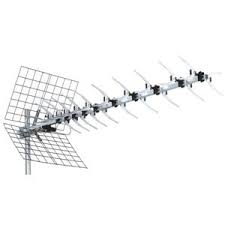
\includegraphics[width=\textwidth]{images/antenne.png}
    \caption{SKT SL43-01 UHF 43 Antenne}\label{antenne}
\end{figure}
\section{Signal}
\subsection{Aufbau von LTE}
\subsubsection{PSS}
\subsubsection{SSS}
\section{Software}

Nachfolgend soll nun die verwendete Softwaresuite erläutert werden. Dazu wird zunächst die zur Aufnahme genutzte Lösung beschrieben. Anschließend wird näher auf die eigens entwickelte Signalverarbeitungskette eingegangen.

\subsection{Aufnahme}

Um Daten vom PlutoSDR zu empfangen bedarf es einer Bediensoftware um den Empfangsprozess zu steuern. Zahlreiche solcher SDR-Anwendungen existieren auf dem Markt, viele davon Open-Source oder als Freeware erhältlich. Der Hersteller selbst, Analog Devices, bietet ein low-level Treiberpaket namens \emph{libiio} (der Name setzt sich zusammen aus dem Unix typischen lib-Präfix für \emph{library} und dem Akronym iio---%
% cspell:disable-next-line
\textbf{i}ndustrial \textbf{i}nput/\textbf{o}utput---%
steht) an. Mit diesem ist es möglich lokal-, über USB- oder Netzwerk verbundene ADCs und FPGAs von Analog Devices zu steuern. Das Treiberpaket beinhaltet dabei einige Kommandozeilenanwendungen mit denen angeschlossene Geräte enumeriert, einzelne Register gelesen und beschrieben und die Firmware ak­tu­a­li­sie­rt werden können. Darüber hinaus kann über eine API, die Teil der namensgebenden libiio Bibliotheksdatei ist, auf Geräte zugegriffen werden.

Es ist diese API an der die meisten SDR-Anwendungen ansetzten. Welche Funktionen der Hardware dann genau nutzbar sind, hängt von der jeweiligen Anwendung ab. Für die Durchführung dieses Projekts würde sich dabei für die Anwendung SDRangel\footnote{Homepage: \url{https://bit.ly/sdrangel}} von Edouard Griffiths entschieden. Abbildung~\ref{fig:sdrangel_screenshot} zeigt die graphische Oberfläche der Anwendung. Die Software unterstützt das Darstellen und Aufzeichnen von IQ-Rohdaten in einem eigenen Dateiformat. Die Möglichkeit der Live-Darstellung der Daten in Frequenz- und Wasserfalldiagramm hat sich in den Messkampagnen als äußerst hilfreich erwiesen.

\begin{figure}[htb]
    \centering
    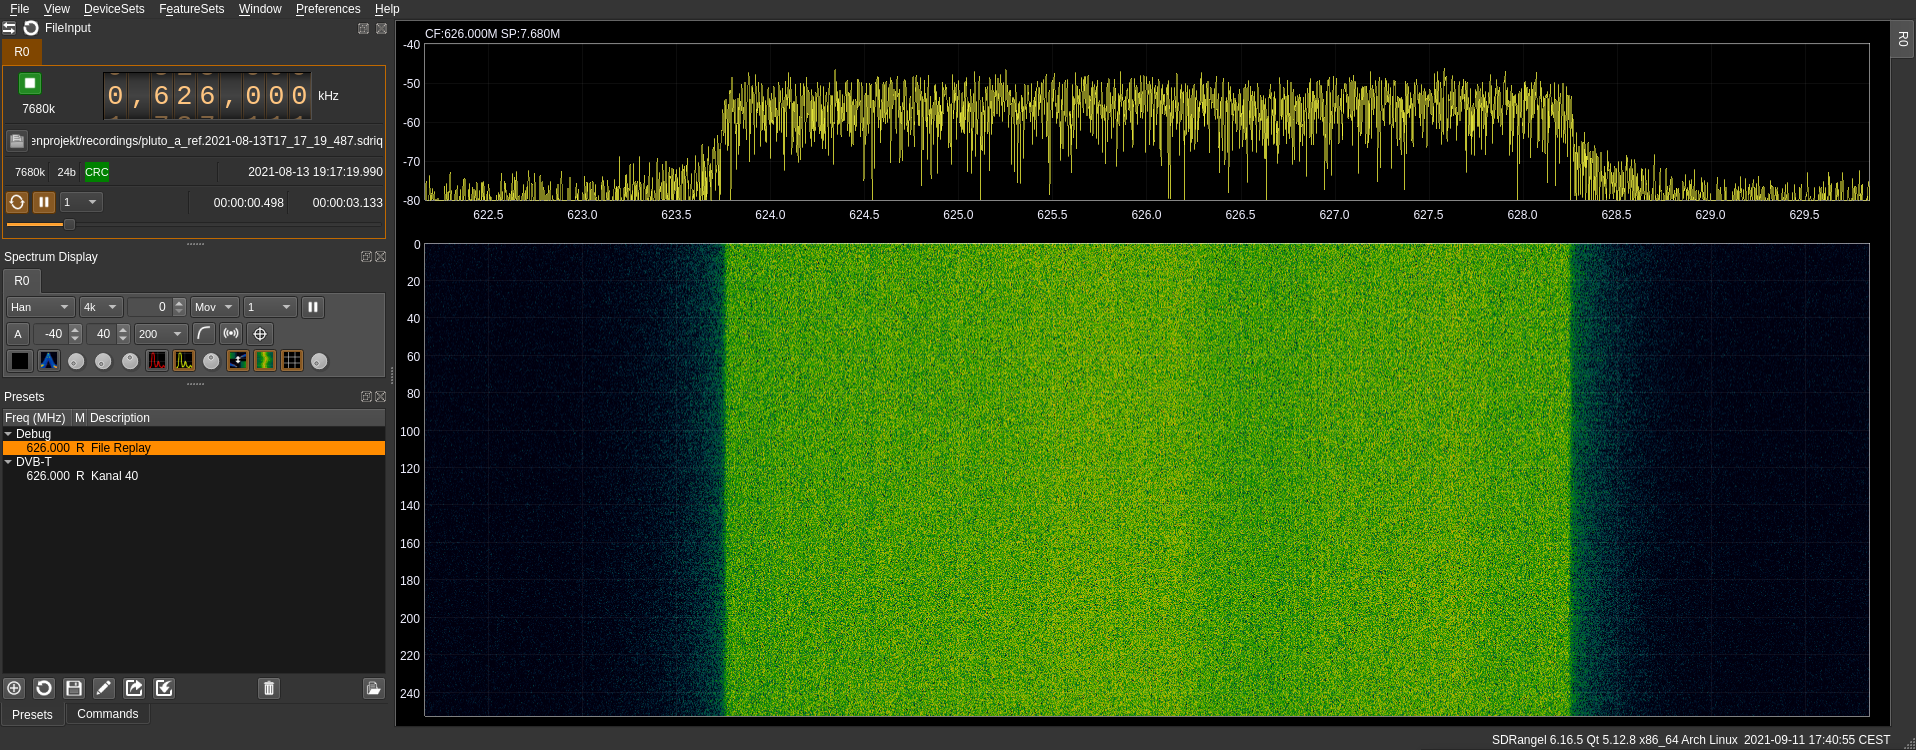
\includegraphics[width=\textwidth]{images/sdrangel.png}
    \caption{SDRangel im Replay-Modus einer zuvor angefertigten Messung.}\label{fig:sdrangel_screenshot}
\end{figure}

Da es sich hierbei um Open-Source-Software handelt, konnten benötigte Funktionen oder Bugfixes\footnote{Liste aller Änderungen: \url{https://bit.ly/sdrangel-pr}} direkt selbst implementiert werden und sind anschließend ins Projekt zurück geflossen. So wurde ein Bugfix zur parallelen Nutzung zweier PlutoSDR erstellt, eingereicht und in den Hauptentwicklungszweig des Ursprungsprojekts aufgenommen.

\subsection{Signalverarbeitung}

Die Signalverarbeitungskette stellt den essenziellen Teil dieser Projektarbeit dar. Bereits zu beginn des Projekts wurde sich dafür entschieden, diese weitestgehend in Python zu implementieren. Als Grundlage für mathematische Operationen dient dabei die numerische Mathematikbibliothek \emph{NumPy}. Zusätzlich wird vereinzelt auf Funktionen der \emph{SciPy-Signal} (Grundbausteine für Funktionen der Signalverarbeitung) oder \emph{CuPy} (GPU-beschleunigte Implementierung der NumPy-Funktionen) Bibliotheken zurückgegriffen. Ziel war es, sich eng vertraut mit den Aspekten der Signalverarbeitung zu machen, und weniger auf vorbereitete Funktionen zurückzugreifen; ohne deren Details zu verstehen. Der Entwicklungsprozess ließ sich dabei grob in zwei Schritte unterteilen. Zunächst wurden Algorithmen prototypisch in Form von Jupyter Notebooks implementiert und getestet. Hier konnten die Methoden und Algorithmen interaktiv entworfen werden, bevor sie im zweiten Schritt in solide und testbare Python Module ausgegliedert wurden.

Die so entstandene Signalverarbeitungskette ist in Abbildung~\ref{fig:signal_processing_chain} gezeigt. Die Direkt- und Echosignale werden über zwei getrennte Kanäle aufgezeichnet. Die beiden Empfänger sind dabei am Wandler phasen- und frequenzkohärent getaktet. Durch die Wandler entsteht ein analytisches Zeitsignal, bestehend aus einer in- und einer \(90^\circ \) verschobenen Phasenkomponente %
% cspell:disable-next-line
(engl.\@ \textbf{I}n-phase und \textbf{Q}uadrature-phase). %
Nach der Wandlung werden diese Daten per USB-Schnittstelle an einen Computer übertragen und dort aufgezeichnet. Dabei ist anzumerken, dass bereits durch die USB-Übertragung jegliche Synchronität der beiden Kanäle verloren geht. Um dem entgegen zu wirken, wird im Dateikopf jeder Aufzeichnung ein Millisekunden genauer Zeitstempel hinterlegt. Da jedoch weder das Betriebssystem noch die Aufnahmesoftware harte Echtzeit unterstützt ist auch hier von mehreren Millisekunden Jitter auszugehen. Um dies zu kompensieren wurde eine Synchronisierungsschnittstelle entworfen, die versucht, die beiden Datenströme zeitlich anzugleichen. Dazu wird zunächst eine grobe Angleichung mittels Zeitstempel aus der Aufzeichnung vorgenommen, anschließend wird versucht über die im LTE Signal enthaltenen Synchronisierungssequenzen eine OFDM-Symbol genaue Synchronisierung herzustellen. So entstehen zwei in Zeit, Frequenz und Phase synchronisierte Datenströme, die für die weitere Prozessierung verwendet werden.

Die mitführung des Referenzkanals ermöglicht grobe Clutter Suppression mittels \emph{CLEAN} Algorithmus~\cite{Kulpa2019}. Dazu soll im Folgenden genauer auf die Kernelemente \emph{CAF} und \emph{CLEAN} eingegangen werden. Finales Ergebnis der Prozesskette ist eine von Clutter bereinigte Range-Doppler Matrix. Zukünftige Arbeiten könnten an dieser Stelle ansetzen und die Informationen aus der Range-Doppler Matrix zur Alarmerzeugung nutzen.

\begin{figure}[htb]
    \centering
    \begin{tikzpicture}[
            flow node/.style={
                    draw,
                    fill=blue!20,
                    rounded corners,
                    minimum height=2em,
                    minimum width=5cm,
                },
            every edge quotes/.style={
                    fill=white,
                    rounded corners,
                    fill opacity=0.8,
                    text opacity=1,
                    font=\scriptsize,
                }
        ]
        \coordinate (origin) at (0,0);

        \node (pluto_a) [flow node, left=0.5cm of origin, anchor=east] {PlutoSDR A};
        \node (pluto_b) [flow node, right=0.5cm of origin, anchor=west] {PlutoSDR B};

        \node (antenna_a) [bareRXantenna, above=1.5cm of pluto_a]{Rx A};
        \node (antenna_b) [bareRXantenna, above=1.5cm of pluto_b]{Rx B};

        \node (recording_ref) [flow node, below=1.5cm of pluto_a, anchor=north] {Aufzeichnung (Ref.)};
        \node (recording_surv) [flow node, below=1.5cm of pluto_b, anchor=north] {Aufzeichnung (Surv.)};

        \node (parser_ref) [flow node, below=1.5cm of recording_ref, anchor=north] {Parser};
        \node (parser_surv) [flow node, below=1.5cm of recording_surv, anchor=north] {Parser};

        \path let \p1=($(parser_ref.south)!0.5!(parser_surv.south)$) in node (sync) [flow node, below=1.5cm of (\p1), anchor=north] {Synchronisation};

        \node (caf) [flow node, below=1.5cm of sync, anchor=north] {CAF};

        \node (clean) [flow node, right=1.5cm of caf, anchor=west] {CLEAN};

        \node (display) [flow node, below=1.5cm of caf, anchor=north] {Anzeige};

        \draw (antenna_a) -- (pluto_a);
        \draw (antenna_b) -- (pluto_b);
        \path (pluto_a) edge [->,"IQ Rohdaten"] (recording_ref);
        \path (recording_ref) edge [->,"\directory{reference.sdriq} Datei"] (parser_ref);
        \path (parser_ref) edge [->,"Zeitsignal"] (sync);
        \path (pluto_b) edge [->,"IQ Rohdaten"] (recording_surv);
        \path (recording_surv) edge [->,"\directory{surveillance.sdriq} Datei"] (parser_surv);
        \path (parser_surv) edge [->,"Zeitsignal"] (sync);
        \path (sync) edge [->,"(2x) Sync. Zeitsignal"] (caf);
        \path let \p1=($(caf.east) + (0,0.2cm)$), \p2=($(clean.west) + (0,0.2cm)$) in (\p1) edge [->,"Range-Doppler Matrix" {right,rotate=40}] (\p2);
        \path let \p1=($(clean.west) - (0,0.2cm)$), \p2=($(caf.east) - (0,0.2cm)$) in (\p1) edge [->,"Bereinigtes Zeitsignal" {right,rotate=-40}] (\p2);
        \path (caf) edge [->,"Range-Doppler Matrix"] (display);
    \end{tikzpicture}
    \caption{Schematische Darstellung der Signalverarbeitungskette.}\label{fig:signal_processing_chain}
\end{figure}

\subsubsection{Ambiguity Funktion}\label{sct:ambiguity_function}

Wie bereits durch die Erläuterung des Messprinzips in Kapitel~\ref{chp:theory_of_operation} beschrieben, basiert die Entfernungsschätzung in Passivradarsystemen auf der zeitlichen Korrelation zwischen Referenz- und Echosignal. Neben dem zeitlichen Versatz, welcher Rückschlüsse auf die Entfernung erlaubt, kann unter Berücksichtigung des Frequenzversatzes beider Signale auch eine bistatische Geschwindigkeit ermittelt werden. Um den Versatz eben dieser beiden Größen bestimmen zu können, wird in der Radartechnik allgemein auf die s.\,g.\ Kreuzambiguitätsfunktion (CAF) zurückgegriffen. Darunter wird die mathematische Korrelation zweier Eingangssignale unter Variation des Zeit- und Frequenzversatzes verstanden. Die resultierende Größe gibt Aufschluss über die \emph{Ähnlichkeit} beider Signale an den gewählten Funktionsparametern. Mathematisch ausgedrückt ist die CAF gegeben durch~\cite[S.~132]{Malanowski2019}:

\begin{equation}\label{equ:cross_ambiguity_function}
    \psi(t, f_{\text{d}}) = \int_{-T/2}^{T/2} {x_{e}(s) \cdot x_{r}^{*}} \left( s - t \right)\mathrm{e}^{\mathrm{j} 2 \pi f_{d} s} \, \text{d} s
\end{equation}

Die Variablen \(t\) und \(f_{d}\) steuern dabei den Zeit- bzw. Frequenzversatz. Die Funktionen \(x_{r}(s)\) und \(x_{e}(s)\) bestimmen das Referenz- bzw. Echosignal im Zeitbereich. \(T\) stellt den Integrationsintervall (auch Coherent Processing Interval [CPI]) dar. \({\{}\cdot{\}}^{*}\) wird hier als Operator der komplexen Konjugation und \(\mathrm{j}\) als imaginäre Einheit genutzt.

Da in der Regel mit digitalen Systemen gearbeitet wird, soll an dieser Stelle auch die zeitdiskrete Variante der CAF eingeführt werden:

\begin{equation}\label{equ:cross_ambiguity_function_digital}
    \psi(m, k) = \sum_{n = 0}^{N - 1}{x_{e}(n) \cdot x_{r}^{*}(n - m) \mathrm{e}^{-\mathrm{j} \frac{2 \pi}{N} k n}}
\end{equation}

Wobei nun \(m\) den Zeitversatz in Samples, \(k\) den Frequenzversatz in Frequency Bins, sowie \(N\) die Anzahl Samples im Integrationsfenster ausdrückt.

In der Praxis wird die CAF für ein ausgewähltes Intervall der Eingangsparameter \(m\) und \(k\) bzw.\@ \(t\) und \(f_\text{d}\) berechnet. Daraus resultiert eine Range-Doppler Map, in der nach potenziellen Zielen, s.\,g.\ Alarmen, gesucht wird. Die Einzelheiten solcher Detektionsalgorithmen, wie z.\,B.\ dem weit verbreitete Constant False Alarm Rate Detector (CFAR)~\cite[S.~208--230]{Malanowski2019}, sind nicht mehr Teil dieser Arbeit. Daher soll zunächst der Fokus auf der CAF bleiben.

Zwar liefert eine direkte Implementierung der Gleichung~\ref{equ:cross_ambiguity_function_digital} mittels gängiger numerischer Basisoperationen bereits das gewünschte Ergebnis, jedoch ist die direkte Berechnung mit erheblicher Zeitkomplexität verbunden. Im Rahmen dieser Projektarbeit wurden daher verschiedene Implementierungen der CAF umgesetzt, auf die im Folgenden kurz eingegangen werden soll. Alle Implementierungen wurden mit einfachen synthetischen Beispielen, sowie gegeneinander getestet.

\begin{description}
    \item[Direkte Implementierung]

          Diese erste Implementierung dient primär als Verifikationswerkzeug der anderen Varianten. Die CAF wird dabei naiv über eine direkte Übersetzung der Gleichung~\ref{equ:cross_ambiguity_function_digital} in numerische Operationen erzielt. Darüber hinaus werden keinerlei Vereinfachungen zur effizienteren Berechnung vorgenommen. Für jedes Eingangspaar \(m\) und \(k\) wird zunächst eine Matrixzeile des entsprechend zeitlich verschobenen Referenzsignals angelegt. Anschließend wird das Schur Produkt des komplex konjugierten und verschobenen Referenzsignals mit dem Echosignal gebildet. Schließlich muss die so entstandene Matrix aus Verzögerungsprodukten nun mit der analog aufgebauten komplexen Doppler-Exponenten Matrix multipliziert werden.

          Ein sich aus dieser Herangehensweise ergebender Vorteil ist die Möglichkeit, beliebige Permutationen der Eingangspaare \(m\) und \(k\) zu bestimmen. Entscheidender Nachteil ist die hohe Zeitkomplexität dieses Algorithmus.
    \item[Fine Mode (CPU)]

          Ein approximativer Algorithmus zur Bestimmung der CAF, erstmals beschrieben in~\cite{Stein1981}. Auszeichnende Charakteristiken sind die verringerte Zeitkomplexität bei relativ geringem Implementierungsaufwand. Eine alternative Herleitungen basieren auf~\cite{Yatrakis2001} und~\cite[S.~135--136]{Malanowski2019} wurde letztendlich implementiert. Die Kernidee basiert auf der Annahme, dass der Dynamikbereich der Dopplerfrequenz deutlich geringer als die Samplerate \(f_{d,max} << F_{s}\) ist. Diese Annahme lässt sich auf das in dieser Arbeit betrachtete Szenario folgendermaßen ausweiten: Mit einer angenommenen maximalen Dopplergeschwindigkeit von \SI{100}{\metre\per\sec} (Flugzeug in Landeanflug) lässt sich der Dynamikbereich durch umstellen der Gleichung~\ref{equ:bistatic_velocity} bestimmen. Somit gilt: % chktex 35
          \begin{equation*}
              f_{d,max} = \left| \SI{624}{\mega\hertz} \cdot \frac{\SI{1000}{\metre\per\sec}}{\SI{3e8}{\metre\per\sec}} \right| \approx \SI{208}{\hertz} << F_s = \SI{5}{\mega\hertz} % chktex 35
          \end{equation*}

          In~\cite{Yatrakis2001} wird basierend auf dieser Ungleichung eine Approximation vorgenommen, die es erlaubt, das Problem in drei Schritten zu lösen. Vereinfacht lauten diese:
          \begin{enumerate}
              \item Berechne das komplexe Produkt zwischen Echo und dem dem um \(\tau \) verzögerten Referenzsignal.
              \item Dezimiere das Verzögerungsprodukt um \(L << F_s / 2 \pi v_{max} \). Wobei \(v_{max}\) die maximal erwartete Dopplergeschwindigkeit in \si{\metre\per\second} darstellt. % chktex 35
              \item Berechne die \(\mathbf{DFT} {\{ \cdot \}}\) des dezimierten Produktes.
          \end{enumerate}

          Abbildung~\ref{fig:caf_fine_mode_schematics} zeigt ein Blockschaltbild des beschriebenen Algorithmus. Die Terme \(x_{r}(n)\) und \(x_{e}(n)\) bilden die Samples des Referenz- bzw. Echosignals, wobei das Echosignal zunächst komplex-konjugiert wird. \(z^{a}\) repräsentiert eine Totzeit um \(a\) Samples. Anschließend werden die Signale multipliziert, woraus sich das Verzögerungsprodukt ergibt. Das gemischte Ergebnis wird durch einen Tiefpassfilter mit einer Grenzfrequenz von \(\nicefrac{1}{L}\) geführt. Danach wird eine Dezimierung der Schrittgröße \(L\) angewendet\footnote{NumPy's \lstinline{decimate} führt sowohl Tiefpassfilterung als auch Dezimierung in einer Operation durch.}. Ziel dieser beiden Operationen ist es, den interessanten Frequenzbereich (gegeben durch \(f_{d,max}\)) auf die gesamte Breite des Spektrums aufzuspreizen. Damit werden die Punkte der nachfolgenden \(\mathbf{DFT} {\{ \cdot \}}\) auf den interessenten Frequenzbereich limitiert, statt sie über die gesamte Bandbreite aufzuteilen. Das Ergebnis der \(\mathbf{DFT} {\{ \cdot \}}\) repräsentiert eine Zeitscheibe der Range/Doppler Matrix. % chktex 35

          Zur Überprüfung auf Korrektheit, wurden die Rechenergebnisse mit denen der Direkten Implementierung verglichen. Entscheidender Vorteil dieser Variante ist die deutlich schnellere Berechnung, dank Nutzung des deutlich effizienteren \(\mathbf{FFT} {\{ \cdot \}}\) Algorithmus.

    \item[Fine Mode (GPU)]

          Eine GPU-optimierte Implementierungen des Fine Mode Algorithmus. Funktionsprinzip und Ablauf sind mit der CPU-Version identisch, jedoch werden sämtliche Operationen auf der GPU ausgeführt.

          In der Praxis hat sich gezeigt, dass diese Variante zwar auf ein einzelnes Integrationsintervall bezogen schneller rechnet, jedoch ist die Prozessierung mehrerer Range-Doppler Matrizen im Batch-Modus schnell durch den geringeren VRAM limitiert.
\end{description}

\begin{figure}[htb]
    \centering
    \begin{tikzpicture}[
        result node/.style={
                draw,
                minimum width=1.75cm,
                minimum height=2em,
                thick,
            },
        function node/.style={
                draw,
                minimum width=2.5cm,
                minimum height=2em,
            },
        mixer node/.style={
                mixer,
                scale=0.5,
            },
        delay node/.style={
                function node,
                minimum width=3em,
            },
        input node/.style={
                draw,
                minimum width=1.5cm,
                minimum height=2em,
                thick,
            },
        ghost/.style={
                inner sep=0,
                outer sep=0,
                minimum width=0,
                minimum height=2em,
                anchor=center,
            },
        -|/.style={to path={-| (\tikztotarget)}},
        |-/.style={to path={|- (\tikztotarget)}}
        ]
        \node [result node] (y0) at (0, 0) {\(\psi (0, \cdot)\)};
        \node [result node, anchor=north, below=0.25cm of y0.south] (y1) {\(\psi (1, \cdot)\)};
        \node [result node, anchor=north, below=0.25cm of y1.south] (y2) {\(\psi (2, \cdot)\)};
        \node [result node, anchor=north, below=0.25cm of y2.south] (yD) {\(\psi (\dots, \cdot)\)};
        \node [result node, anchor=north, below=0.25cm of yD.south] (yN) {\(\psi (M, \cdot)\)};

        \node [function node, anchor=east, left=0.25cm of y0.west] (dft0) {\(\mathbf{DFT} {\{ \cdot, L \}}\)};
        \node [function node, anchor=east, left=0.25cm of y1.west] (dft1) {\(\mathbf{DFT} {\{ \cdot, L \}}\)};
        \node [function node, anchor=east, left=0.25cm of y2.west] (dft2) {\(\mathbf{DFT} {\{ \cdot, L \}}\)};
        \node [function node, anchor=east, left=0.25cm of yD.west] (dftD) {\(\mathbf{DFT} {\{ \cdot, L \}}\)};
        \node [function node, anchor=east, left=0.25cm of yN.west] (dftN) {\(\mathbf{DFT} {\{ \cdot, L \}}\)};

        \path (dft0) edge [->] (y0);
        \path (dft1) edge [->] (y1);
        \path (dft2) edge [->] (y2);
        \path (dftD) edge [->] (yD);
        \path (dftN) edge [->] (yN);

        \node [function node, anchor=east, left=0.25cm of dft0.west] (dec0) {\(\mathbf{DEC} {\{ \cdot, L \}}\)};
        \node [function node, anchor=east, left=0.25cm of dft1.west] (dec1) {\(\mathbf{DEC} {\{ \cdot, L \}}\)};
        \node [function node, anchor=east, left=0.25cm of dft2.west] (dec2) {\(\mathbf{DEC} {\{ \cdot, L \}}\)};
        \node [function node, anchor=east, left=0.25cm of dftD.west] (decD) {\(\mathbf{DEC} {\{ \cdot, L \}}\)};
        \node [function node, anchor=east, left=0.25cm of dftN.west] (decN) {\(\mathbf{DEC} {\{ \cdot, L \}}\)};

        \path (dec0) edge [->] (dft0);
        \path (dec1) edge [->] (dft1);
        \path (dec2) edge [->] (dft2);
        \path (decD) edge [->] (dftD);
        \path (decN) edge [->] (dftN);

        \node [function node, anchor=east, left=0.25cm of dec0.west] (lpf0) {\(\mathbf{LPF} {\{ \cdot, \nicefrac{1}{L} \}}\)};
        \node [function node, anchor=east, left=0.25cm of dec1.west] (lpf1) {\(\mathbf{LPF} {\{ \cdot, \nicefrac{1}{L} \}}\)};
        \node [function node, anchor=east, left=0.25cm of dec2.west] (lpf2) {\(\mathbf{LPF} {\{ \cdot, \nicefrac{1}{L} \}}\)};
        \node [function node, anchor=east, left=0.25cm of decD.west] (lpfD) {\(\mathbf{LPF} {\{ \cdot, \nicefrac{1}{L} \}}\)};
        \node [function node, anchor=east, left=0.25cm of decN.west] (lpfN) {\(\mathbf{LPF} {\{ \cdot, \nicefrac{1}{L} \}}\)};

        \path (lpf0) edge [->] (dec0);
        \path (lpf1) edge [->] (dec1);
        \path (lpf2) edge [->] (dec2);
        \path (lpfD) edge [->] (decD);
        \path (lpfN) edge [->] (decN);

        \node [mixer node, anchor=east, left=0.25cm of lpf0.west] (mixer0) {};
        \node [mixer node, anchor=east, left=0.25cm of lpf1.west] (mixer1) {};
        \node [mixer node, anchor=east, left=0.25cm of lpf2.west] (mixer2) {};
        \node [mixer node, anchor=east, left=0.25cm of lpfD.west] (mixerD) {};
        \node [mixer node, anchor=east, left=0.25cm of lpfN.west] (mixerN) {};

        \path (mixer0.east) edge [->] (lpf0);
        \path (mixer1.east) edge [->] (lpf1);
        \path (mixer2.east) edge [->] (lpf2);
        \path (mixerD.east) edge [->] (lpfD);
        \path (mixerN.east) edge [->] (lpfN);

        \node [delay node, anchor=east, left=0.25cm of mixer0.west] (delay0) {\(z^{0}\)};
        \node [delay node, anchor=east, left=0.25cm of mixer1.west] (delay1) {\(z^{-1}\)};
        \node [delay node, anchor=east, left=0.25cm of mixer2.west] (delay2) {\(z^{-2}\)};
        \node [delay node, anchor=east, left=0.25cm of mixerD.west] (delayD) {\(z^{-\dots}\)};
        \node [delay node, anchor=east, left=0.25cm of mixerN.west] (delayN) {\(z^{-M}\)};

        \path (delay0.east) edge [->] (mixer0.west);
        \path (delay1.east) edge [->] (mixer1.west);
        \path (delay2.east) edge [->] (mixer2.west);
        \path (delayD.east) edge [->] (mixerD.west);
        \path (delayN.east) edge [->] (mixerN.west);

        \node [input node, anchor=east, left=0.5cm of delay0.west] (ref) {\(x_{r}(n)\)};
        \node [input node, anchor=south, above=0.25cm of ref.north] (surv) {\(x_{e}^{*}(n)\)};

        \node [ghost, left=0.25cm of delay0.west] (ref_ghost_delay0) {};
        \node [ghost, left=0.25cm of delay1.west] (ref_ghost_delay1) {};
        \node [ghost, left=0.25cm of delay2.west] (ref_ghost_delay2) {};
        \node [ghost, left=0.25cm of delayD.west] (ref_ghost_delayD) {};
        \node [ghost, left=0.25cm of delayN.west] (ref_ghost_delayN) {};

        \path (ref_ghost_delay0.center) edge [->] (delay0.west);
        \path (ref_ghost_delay1.center) edge [->] (delay1.west);
        \path (ref_ghost_delay2.center) edge [->] (delay2.west);
        \path (ref_ghost_delayD.center) edge [->] (delayD.west);
        \path (ref.east) edge [-|] (ref_ghost_delayN.center) (ref_ghost_delayN.center) edge [->] (delayN.west);

        \node [ghost, left=0.125cm of ref_ghost_delay0.center] (surv_ghost0_mixer0) {};
        \node [ghost, left=0.125cm of ref_ghost_delay1.center] (surv_ghost0_mixer1) {};
        \node [ghost, left=0.125cm of ref_ghost_delay2.center] (surv_ghost0_mixer2) {};
        \node [ghost, left=0.125cm of ref_ghost_delayD.center] (surv_ghost0_mixerD) {};
        \node [ghost, left=0.125cm of ref_ghost_delayN.center] (surv_ghost0_mixerN) {};

        \node [ghost, above=0.125cm of surv_ghost0_mixer0.north, minimum height=0] (surv_ghost_mixer0) {};
        \node [ghost, above=0.125cm of surv_ghost0_mixer1.north, minimum height=0] (surv_ghost_mixer1) {};
        \node [ghost, above=0.125cm of surv_ghost0_mixer2.north, minimum height=0] (surv_ghost_mixer2) {};
        \node [ghost, above=0.125cm of surv_ghost0_mixerD.north, minimum height=0] (surv_ghost_mixerD) {};
        \node [ghost, above=0.125cm of surv_ghost0_mixerN.north, minimum height=0] (surv_ghost_mixerN) {};

        \path (surv_ghost_mixer0.center) edge [-|,->] (mixer0.north);
        \path (surv_ghost_mixer1.center) edge [-|,->] (mixer1.north);
        \path (surv_ghost_mixer2.center) edge [-|,->] (mixer2.north);
        \path (surv_ghost_mixerD.center) edge [-|,->] (mixerD.north);
        \path (surv.east) edge [-|] (surv_ghost_mixerN.center) (surv_ghost_mixerN.center) edge [-|,->] (mixerN.north);

        \path (y0.south west) edge [dotted] (y1.north west)
        (y1.south west) edge [dotted] (y2.north west)
        (y2.south west) edge [dotted] (yD.north west)
        (yD.south west) edge [dotted] (yN.north west);
        \path (y0.south east) edge [dotted] (y1.north east)
        (y1.south east) edge [dotted] (y2.north east)
        (y2.south east) edge [dotted] (yD.north east)
        (yD.south east) edge [dotted] (yN.north east);

        \path (y0.north east) -- node [midway,anchor=north,rotate=90] {\tiny Entfernung} (yN.south east);
        \path (yN.south west) -- node [midway,anchor=north] {\tiny Doppler} (yN.south east);
    \end{tikzpicture}

    \caption{Blockdiagramm des Fine Mode CAF Algorithmus.\label{fig:caf_fine_mode_schematics}}
\end{figure}

\subsubsection{CLEAN Algorithmus}

Eine entscheidende Hürde in der Entwicklung eines jeden Radarsystems ist es, gewünschte Signale (s.\,g.\ Targets) von unerwünschten (s.\,g.\ Clutter) zu unterscheiden. Selbstverständlich unterscheidet sich welche Reflexionen als Targets oder als Clutter klassifiziert werden je nach Anwendungsfall. Im Falle eines Luftüberwachungsradars werden üblicherweise nur Reflexionen an Flugzeugen als erwünscht angesehen. Neben diesen, empfangen solche Systeme unweigerlich auch Reflexionen an Terrain, Gebäuden, Wolken, Vogelschwärmen, Bodenfahrzeugen oder Schiffen. Diese Clutter-Quellen unterscheiden sich jeweils in ihrem Radarquerschnitt und somit der Leistung, die sie an einen Empfänger zurückwerfen können. Eine besondere Clutter-Quelle speziell bei Passivradar ist das Einleuchten des Direktsignals, bspw.\ über Nebenkeulen der Empfangsantenne. Dies trifft typischerweise mit deutlich höherer Leistung als die Echos der Targets am Empfänger ein. Es ist daher essenziell, diese und andere Quellen von Clutter zu unterdrücken; man spricht von s.\,g.\ Clutter-Suppression. Ohne jegliche Form von Unterdrückung werden Zielreflexionen meist komplett vom Clutter verdeckt und sind unmöglich in der Range-Doppler Map auszumachen. Für den Prozess der Clutter-Suppression werden typischerweise adaptive Filter verwendet, einige verbreitete Ansätze sind in~\cite[S.~177--202]{Malanowski2019} beschrieben.

Aufgrund der einfachen Implementierung wird in dieser Projektarbeit der CLEAN Algorithmus zur Clutter-Suppression eingesetzt. Damit wird in der aktuellen Version vornehmlich versucht, die Direkteinstrahlung des Referenzsignals im Überwachungskanal zu unterdrücken. Diese Anwendung wurde unter anderem in~\cite{Feng2013} demonstriert.

Der Funktion des CLEAN Algorithmus liegt folgendes an~\cite{Kulpa2008} angelehnte Empfangsmodell zugrunde. Zunächst wird ein Referenz- und ein Überwachungskanal im Basisband definiert. Der Referenzkanal wird als die gedämpfte und mit additivem weißen Rauschen \(\eta (t)\) beaufschlagte Senderwellenform \(u (t)\) modelliert:
%
\begin{equation}
    y_{ref} (t) = a \cdot u (t) + \eta_{ref} (t)
\end{equation}\label{equ:clean_reference_channel}%
%
Wobei \(a\) die nach Dämpfung verbleibende komplexe Amplitude des Signals darstellt.

Im Überwachungskanal wird diese Wellenform als Summe von \(n\) Reflexion an stationären oder bewegten Objekten behandelt. Die aufgrund der Mehrwegeausbreitung verlängerte Signallaufzeit vom \(i\)-ten Objekt zum Empfänger wird als zum Referenzsignal relativer Zeitversatz \(\tau_{i} \) aufgespielt. Gleichermaßen wird ein Dopplerversatz \(f_{d,i}\) für bewegte Ziele beaufschlagt. Schließlich ist auch der Überwachungskanal einem weißen Rauschen ausgesetzt:%
%
\begin{equation}
    y_{surv} (t) = \sum_{i = 0}^{n}{a_{i} \cdot u (t - \tau_{i}) \cdot \mathrm{e}^{\mathrm{j} 2 f_{d,i} t}} + \eta_{surv} (t)
\end{equation}%
%
Wobei \(\mathrm{j}\) die imaginäre Einheit darstellt. Die so modellierten \(i\) Kopien der vom Sender emittierten Wellenform können sowohl erwünschte Zielreflexionen aber auch Clutter oder Direkteinstrahlung des Referenzsignals sein. Es ist davon auszugehen, dass Direkteinstrahlung und Clutter höhere Amplitude aufweisen, als echte Ziele. Diese werden somit von den unerwünschten Reflexionen \emph{überleuchtet}. Ziel ist es nun, die Parameter \(a_{i}\), \(\tau_{i}\) und \(f_{d,i}\) eben dieser unerwünschten Einstrahlungen zu schätzen, um im nächsten Schritt entsprechend zeit- und frequenzverschobene Senderwellenform vom Überwachungskanal abzuziehen. Übrig bleiben die Reflexionen der erwünschten Ziele.

Die Kernidee des CLEAN Algorithmus besteht nun darin, die genannten Parameter aus den Peaks der Range/Doppler Matrix abzulesen und rekursiv vom Überwachungskanal abzuziehen. Dabei basiert die Entscheidung, welche Peaks Ziele und welche Clutter darstellen, auf a priori Wissen über das Operationsgebiet. Vorausgesetzt Sender, sowie Empfänger sind stationär; und beide Empfangsantennen in unmittelbarer Nähe zueinander, so ist beispielsweise davon auszugehen, dass der höchste Peak vom Direktsignal bei \(\tau_{direct} \approx 0\) und \(f_{d,direct} \approx 0\) ausgeht. Was fehlt ist die komplexe Amplitude, die aus dem verschobenen Referenzsignal bezogen werden kann. Vor der Subtraktion vom Überwachungskanal, ist sicherzustellen, dass sowohl das geschätzte Clutter-Signal als auch der Überwachungskanal normiert sind.

Das eingeführte Empfangsmodell wird in Abbildung~\ref{fig:clean_signal} demonstriert. Als Senderwellenform dient hier eine gepulste Sinuswelle, dargestellt in~\ref{fig:clean_base_waveform}. Diese geht leicht gedämpft über den Referenzkanal zuzüglich Rauschen am Empfänger ein, und erzeugt das in~\ref{fig:clean_ref_waveform} gezeigte Bild. Der rot markierte Bereich hebt das Direktsignal hervor. Abbildung~\ref{fig:clean_surv_waveform} zeigt den Überwachungskanal. Auch hier leuchtet das Direktsignal ein, allerdings über eine Antennennebenkeule und somit stärker gedämpft als im Referenzkanal. Zusätzlich wird --- im Bild blau hinterlegt --- das schwache Echo eines Ziels empfangen.

\begin{figure}[htb]
    \centering
    \subcaptionbox{Ausgesendete Wellenform\label{fig:clean_base_waveform}}{
        \includesvg[width=0.9\textwidth]{images/generated/clean_base_waveform.svg}
    }

    \subcaptionbox{Empfangenes Signal im Referenzkanal\label{fig:clean_ref_waveform}}{
        \includesvg[width=0.9\textwidth]{images/generated/clean_ref_waveform.svg}
    }

    \subcaptionbox{Empfangenes Signal im Übertragungskanal\label{fig:clean_surv_waveform}}{
        \includesvg[width=0.9\textwidth]{images/generated/clean_surv_waveform.svg}
    }
    \caption{Empfangsmodell des CLEAN Algorithmus}\label{fig:clean_signal}
\end{figure}

Abbildung~\ref{fig:clean_amb_before_2d} schließlich zeigt die aus Referenz- und Übertragungskanal resultierende CAF\@. Zu erkennen ist die starke Einwirkung des Direktsignals auf die Kreuzambiguitätsfunktion. Das damit verglichen schwache Ziel ist nur noch schwer auszumachen. Die dreidimensionale Darstellung der gleichen CAF in~\ref{fig:clean_amb_before_3d} zeigt dies noch einmal eindrücklich. Abbildung~\ref{fig:clean_amb_after_2d} und~\ref{fig:clean_amb_after_3d} zeigen nun die CAF nach einmaliger Anwendung des CLEAN Algorithmus. Gut erkennbar ist die starke Reduktion des Direktsignals, übrig bleibt das Zielecho und der umgebene Rauschteppich.

\begin{figure}[htb]
    \centering

    \subcaptionbox{2D vor CLEAN\label{fig:clean_amb_before_2d}}{
        \includesvg[width=0.6\textwidth]{images/generated/clean_amb_before_2d.svg}
    }%
    %
    \subcaptionbox{3D vor CLEAN\label{fig:clean_amb_before_3d}}{
        \includesvg[width=0.3\textwidth]{images/generated/clean_amb_before_3d.svg}
    }

    \subcaptionbox{2D nach CLEAN\label{fig:clean_amb_after_2d}}{
        \includesvg[width=0.6\textwidth]{images/generated/clean_amb_after_2d.svg}
    }%
    %
    \subcaptionbox{3D nach CLEAN\label{fig:clean_amb_after_3d}}{
        \includesvg[width=0.3\textwidth]{images/generated/clean_amb_after_3d.svg}
    }
    \caption{Anwendung des CLEAN Algorithmus}\label{fig:clean_application}
\end{figure}

Die bisher besprochene Form des CLEAN Algorithmus geht davon aus, dass die Senderwellenform bekannt ist, und rauschfrei synthetisiert werden kann. In der Praxis geschieht dies bei Digitalsignalen zumeist durch Demodulation und Dekodierung des Referenzkanals~\cite{Feng2013}. Da dieser Ansatz jedoch mit erheblichem Aufwand verbunden ist, setzt diese Projektarbeit auf eine weniger zeitaufwendige Alternative. So wird stattdessen das Referenzsignal als beste verfügbare Approximation der ursprünglichen Senderwellenform genutzt. Damit einhergehend ist von reduzierter Clutter-Suppression Performance auszugehen, da Referenz- und Überwachungskanal möglicherweise unterschiedlicher Rauschcharakteristiken ausgesetzt sind. Zudem kann die Anwendung der Direktpfadunterdrückung auch zur Dämpfung erwünschter Ziele führen, da die in Gleichung~\ref{equ:clean_reference_channel} getroffene Annahme über den Referenzkanal nur bedingt anwendbar ist. Grund hierfür sind die Antennennebenkeulen die bei jeder realen Antenne auftreten. Über diese werden unweigerlich auch Echosignale gewünschter Ziele ins Referenzsignal eingeschleust. Die Subtraktion des Direktsignals vom Überwachungskanal kann dann auch zur Dämpfung eben dieser Ziele führen. Hier liegt Potenzial für weiterführende Arbeiten, die mit besser geeigneten Clutter-Suppression Techniken ansetzen könnten.

\include{report/durchführung}
\chapter{Ergebnisse \& Ausblick}

In diesem Kapitel werden die Ergebnisse des Studienprojekts präsentiert. Dabei ist zu beachten, dass die in der Einleitung getroffenen Zielvorgaben nur teilweise erfüllt werden konnten. Dafür soll zunächst ein Fazit der faktisch vorhandenen Funktionalität gezogen werden. In der darauffolgenden Diskussion der Ergebnisse soll besonderer Fokus auf die vermuteten Problemquellen gelegt werden. Dies soll Ansatzpunkte für mögliche Verbesserungen in zukünftigen Arbeiten geben.

\section{Projektfazit}

Untersucht wurde die Machbarkeit der Nutzung eines regionalen LTE-basierten 5G Broadcast-Signals als Illuminator of Opportunity unter Verwendung preisgünstiger und leicht erhältlicher Elektronik-Hardware, sowie freier Software in einem selbstentworfenen Passivradar-System. Das 5G Broadcast-Signal wurde auf praktische Aspekte der Nutzung als Beleuchter untersucht und eine entsprechende Signalverarbeitungskette implementiert. Mehrere Iterationen des Hardware-Aufbaus wurden durchgeführt, um den Anforderungen an Bandbreite und Synchronität gerecht zu werden. Zum Aufzeichnen der Daten wurden Fehlerbehebungen in frei verfügbarer Open-Source-Software durchgeführt, und diese Änderungen zurück an den Maintainer übergeben. Zusätzlich wurden weitere Verbesserungen in Zeitstempelgenauigkeit, sowie Anwendungsstabilität vorgenommen, und ebenfalls in die öffentliche Code-Basis eingespielt. Über den Zeitrahmen des Projekts wurden mehrere Messkampagnen im Feld durchgeführt. Die aufgezeichneten Daten dienten zur Weiterentwicklung der Signalverarbeitungskette im Labor. Durch Prozessierung konnten theoretisch besprochene Eigenschaften des LTE-Signals nachgewiesen und zur Signalsynchronisierung genutzt werden. Eigene Algorithmen zur Bestimmung der Kreuzambiguität und Anwendung von Clutter-Suppression wurden implementiert. Deren individuelle Funktionalität wurde durch einfache Tests geprüft und bestätigt. Nichtsdestotrotz scheiterte der beschriebene Aufbau in der Detektion landender und startender Flugzeuge.

\section{Diskussion}

Nachfolgend sollen mögliche technische Ursachen zur Nichterfüllung des Projektziels diskutiert werden. Die Reihenfolge orientiert sich dabei grob an der in Abschnitt~\ref{sct:software} besprochenen Prozesskette.

\subsection{Hardware}

Ein Aspekt, auf den in dieser Projektarbeit besonderer Wert gelegt wurde, ist die Synchronität der Datenströme. Das Gleichschalten der lokalen Oszillatoren über kurze Leitungen zu beiden PlutoSDRs ermöglicht Nanosekunden-synchrones Sampling der ADCs, auch wenn diese Überlegung nie überprüft wurde. Die Synchronität geht jedoch verloren, sobald die Daten über USB an den Host-PC übertragen werden. Die verlorene Synchronität muss dann aufwendig über im Host erzeugte Zeitstempel, welche aufgrund der fehlenden Echtzeitfähigkeit des Betriebssystems um mehrere Mikro- bis Millisekunden variieren können, wiederhergestellt werden.

Sollte höhere Synchronität in weiterführenden Arbeiten erforderlich werden, könnte dementsprechende Funktionalität über Änderungen an der PlutoSDR Firmware umgesetzt werden. Genauere Zeitstempel wären über Anpassungen an der Firmware des auf dem PlutoSDR verbauten Xilinx Zynq FPGAs möglich.

\subsection{Aufnahme}

Ein im Offline-Test der Aufnahmesoftware entdecktes Problem ist der Verlust von Samples beim Aufzeichnen mit hoher Bandbreite. Es besteht die Möglichkeit, dass dieses Problem auch in den Feldmessungen aufgetreten ist, jedoch durch die Umstände der Messung unbemerkt blieb. Im Format der vorliegenden Messdaten sind keinerlei Metadaten zu während der Messung aufgetretenen Fehlern vorgesehen. Die Software meldet den Verlust von Samples lediglich über die Standard-Ausgabe auf einem möglicherweise angeschlossenen Terminal. Da die Software bei den Feldmessungen allerdings nicht aus einem Terminal, sondern über die GUI gestartet wurde, blieben mögliche Hinweise auf verlorene Datenpakete unbemerkt. Offline-Tests haben ebenfalls gezeigt, dass Sample-Verlust, durch Auslastung der CPU (bspw\@. durch parallele Betrachtung im Wasserfalldiagramm) begünstigt wird. Da dieses Phänomen erst gegen Projektende und nach Abschluss aller Messkampagnen bemerkt wurde, konnten keine neuen Messungen erhoben werden.

Weiterführende Arbeiten sollten sicherstellen, dass keine Samples bei der Messung verloren gehen. Außerdem sollten Mechanismen, wie visuelles Feedback über auftretende Fehler bei der Messung, implementiert werden.

\subsection{Synchronisation}

Da die Software ausschließlich für den Offlinebetrieb mit aufgezeichneten Daten ausgelegt ist, müssen die versetzt gestarteten Aufzeichnungen zunächst durch ein Synchronisierungsmodul präprozessiert werden. Da die Aufnahmen während der Feldmessung händisch gestartet werden, müssen so einige Sekunden Zeitunterschied angeglichen werden. Bereits ein Zeitversatz von \SI{1}{\milli\second} entspräche einer bistatischen Distanz von \SI{100}{\kilo\metre}. Ein höherer Versatz könnte dafür sorgen, dass der sich überschneidende Signalteil außerhalb des evaluierten bistatischen Entfernungsintervalls liegt. Des Weiteren wäre eine blinde Suche nach dem statischen Zeitversatz mittels Kreuzambiguität durch \emph{falsche} Peaks resultierend aus Nebenkeulen der Autoambiguität erschwert. Aus diesem Grund wird in dieser Projektarbeit eine Zwei-Stufen Synchronisation basierend auf Zeitstempeln und PSS-Sequenzen durchgeführt. Letztere hat sich jedoch als oft fehlerhaft und wenig verlässlich erwiesen. Abbildung~\ref{fig:pss_correlation_results} zeigt die Korrelationsergebnisse aller drei PSS Sequenzen über jeweils den Referenz- und Überwachungskanal. Die Daten stammen aus unter realbedingungen ausgeführten Feldmessungen, in der beide Antennen parallel in Richtung Beleuchter ausgerichtet wurden. Die y-Achsen sind auf den hochsten Peak aller drei Sequenzen normiert. Zu erkennen ist, dass die in Rot hervorgehobene zweite Sequenz deutlich erkennbare Peaks aufweist. Jedoch zeigen diese Peaks nicht die Regularität, die bei einem MBMS-LTE Signal zu erwarten wäre.

\begin{figure}[htb]
    \centering
    \includesvg[width=\textwidth]{images/generated/pss_correlation_results.svg}
    \caption{Ergebnisse der PSS-Korrelation von Referenz- und Überwachungskanal.}\label{fig:pss_correlation_results}
\end{figure}

\subsection{Clutter-Suppression}

Zur Clutter- und Direktsignalunterdrückung wird der CLEAN Algorithmus eingesetzt. Ausgewählt wurde dieser vornehmlich aufgrund seiner einfachen Funktionsweise und Implementierung. Ob der CLEAN Algorithmus im gegebenen Szenario die gewünschte Clutter-Suppression Performance liefert, konnte aus zeitlichen Gründen nicht hinreichend innerhalb dieser Projektarbeit evaluiert werden. Hierfür sind weitere Analysen notwendig. Aufgrund der beschränkten Informationen über öffentliche 5G Sendeanlagen müssen viele Protokollparameter gemessen oder erraten werden. So basieren viele der in dieser Projektarbeit eingesetzten Verarbeitungsschritte auf Annahmen, die nicht mit dem Betreiber abgesprochen, oder, aufgrund fehlendem professionellem Messequipments, durch eigene Messungen bestätigt werden konnten. Es besteht somit keine solide Basis, mit der die selbst bestimmten Eigenschaften verglichen werden können, was auf den Projekterfolg allgemein bezogen hinderlich wirkt.

\printbibliography % chktex 1

\end{document}
